\documentclass[a4paper, 11pt]{article}
\usepackage{graphicx}
\usepackage{algorithm}
\usepackage{algpseudocode}
\usepackage{amsmath}
\usepackage{tikz}

%\usepackage[a4paper,top=2cm,bottom=2cm,left=2.4cm,right=2.4cm]{geometry}

\usepackage{listings}

\title { Interactive Graphics Project\\ \bigskip \large IG Sapienza}
\date{22 September 2019}
\author{Silvio Dei Giudici 1708962 , \\Marco Morella 1693765, \\Fortunato Tocci 1695457}

\begin{document}
\maketitle

\section{Introduction}
This paper is a descriptive companion to our final project for the Interactive Graphic course.\\
We made a clone of one of the precursor to the modern mobile games, because it had all the prerequistes we were asked to fullfil and it looked like a fun challenge. In the following, we are going to talk about the user aspect of the game as well as all the technical aspect and the challenges we had to deal with. We divided evenly the work weight between all the members while giving support to each other.\\
The end result was a good looking playable game with all the features we wanted during the designing period(and more).
\newpage

\section{User Manual}
\subsection{Commands and User Interface elements}
In this section we are going to analyze everything the user can do in our game.\\
Starting from the home page the user can either:
\begin{itemize}
\item Play: which will bring to the options to pick before being able to play.
\item Commands: which will bring up the following screen showing which movement the user can do when playing.
\begin{center}
	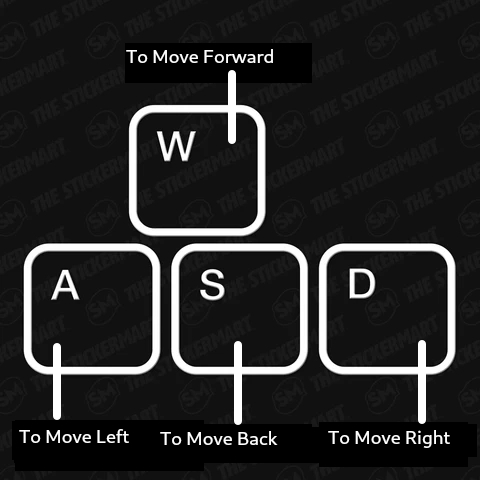
\includegraphics[width = 5cm]{commads.jpg}\\
\end{center}
\item Credits: brings to a page stating all the students involved in the project.
\end{itemize}
After hitting play, the user is presented with a page where he can select:
\begin{itemize}
\item Character: which of the three animals he wants to use. All animals jump the same distance in the same amount of time, in order to not give any of them advantage over the others. In the first draft, the fox jumped longer, the chicken jumped higher and descended slower.
\item Day/Night: either play with the sun as the light source, or a lamp post.
\item Difficulty: pick the level of difficulty of the game, Easy/Medium/Hard.
\end{itemize}
In game, on the upper side we will see the high score and current score reached during this run.\\
On the upper right a button will pause the game and a menu will pop up where the user can either resume the game or go back to the starting page.\\
Clicking the upper left button will change the light from day to night and vice-versa.
\subsection{How to play}
The goal of the user is to help the animal cross the streets and the rivers to reach the safe grass field on the other side avoiding all the dangerous drivers. But if the animal goes outside the viewable area, it will get lost and it's game over!\\
Also, the animal has no idea how to swim across and neither has any airbags, so getting in the river or being hit by a car is game over!

%TECHNICAL PART
\section{Development environment}
\subsection{WebGL}
%parla delle cose che stanno nelle slide eventualmente (un riassuntino), tipo vertex e fragment shader, come si rappresentano oggetti (vertici)
%come rappresentare movimenti (con matrici ecc)
\subsection{Library and tools}
The tools we used were:
\begin{itemize}
\item Three.js: a library that simplifies the interaction between the programmer and WebGL, this was used to create the scene with all the objects in it, perform the movements of the animations, create the lights and shadows and add the textures.
\item OrbitControls: a sub library of three.js used to control the camera movement, which was extremely useful to check if the game was behaving correctly.
\item Browser firefox and its built-in console: to test the project during the developing using logs and alerts.
\item Atom: it was the IDE picked by the group to code. We wanted to uniform it since some IDEs indentation is not compatible with all other IDEs.
\item Github: we've used Github to share the code between the group, see the commits on the repository, check the difference between versions.
\end{itemize}
\newpage
\section{Technical Solutions}
In order to better understand some of what we will discuss later, we want to introduce the directions that are seen in the game:\\
\begin{center}
	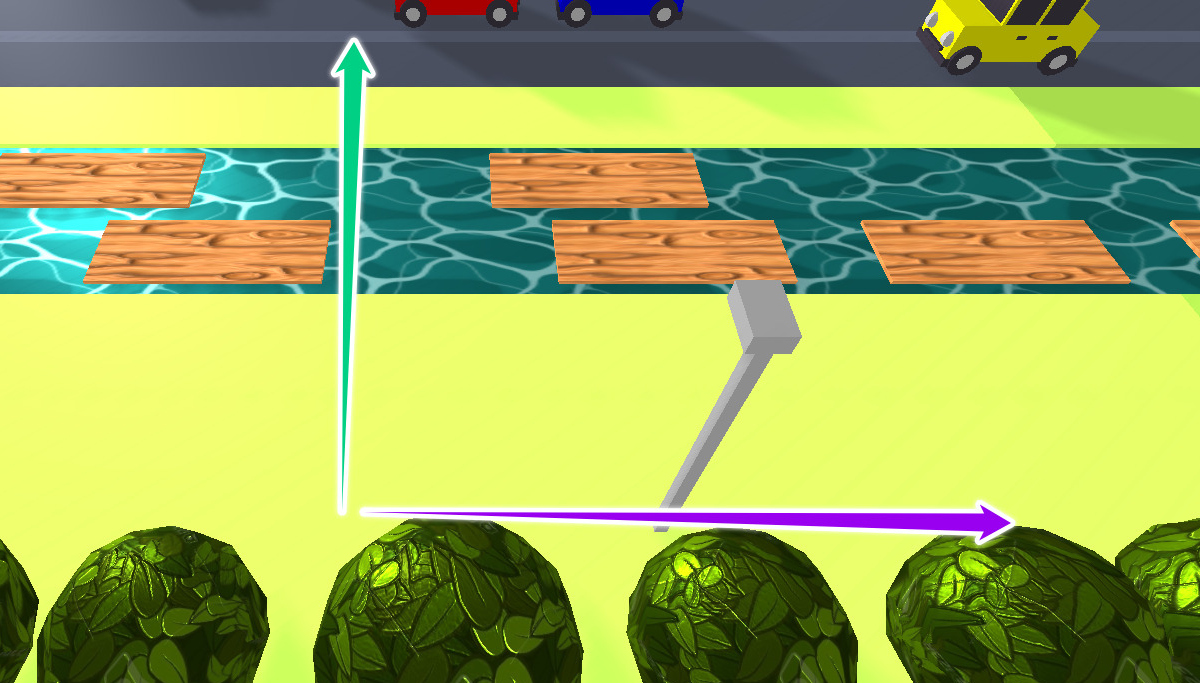
\includegraphics[width =\linewidth]{axis.jpg}\\
\end{center}
The green arrow represents the positive direction of the Z axis, while the purple one represents the positive direction of the X axis.\\ The Y axis is trivially the direction from the ground.
\subsection{Hierarchical models}
We will now analyze all hierarchical models used in the project.
\subsubsection{Animals}
We will only analyze the most complex hierarchical animal model, the fox, since the other two are similar and easier.\\
This is the graph of the final model, to avoid cluttering, i've defined as Face Details all son nodes of head: both ears, both eyes and the nose, which are all brothers.\\
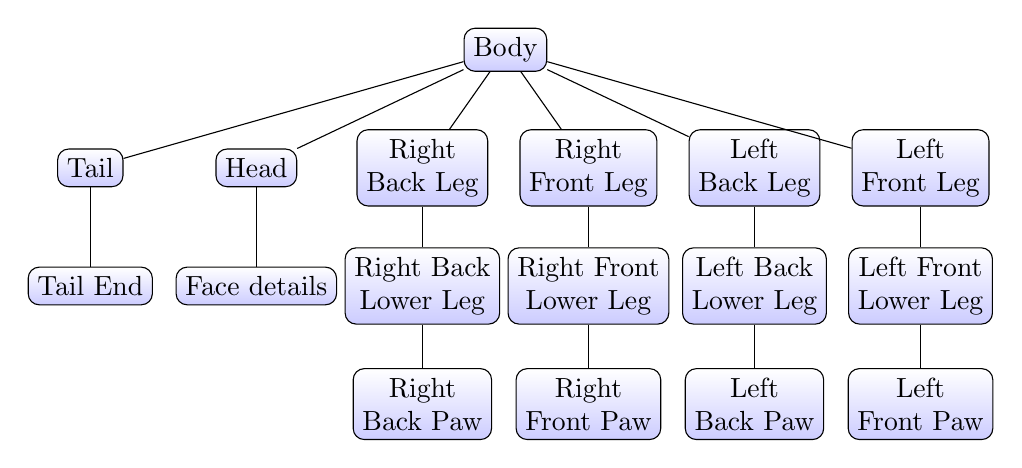
\begin{tikzpicture}[sibling distance=6em,
  every node/.style = {shape=rectangle, rounded corners,
    draw, align=center,
    top color=white, bottom color=blue!20}]]
  \node {Body}
    child { node {Tail}
      child { node {Tail End} }}
    child { node {Head}
      child { node {Face details} }}
    child { node {Right\\Back Leg}
      child { node {Right Back\\Lower Leg}
        child { node {Right\\Back Paw} } }}
    child { node {Right\\Front Leg}
      child { node {Right Front\\Lower Leg}
        child { node {Right \\Front Paw} } }}
    child { node {Left\\Back Leg}
      child { node {Left Back\\Lower Leg}
        child { node {Left\\Back Paw} } }}
    child { node {Left \\Front Leg}
      child { node {Left Front\\Lower Leg}
        child { node {Left\\Front Paw} } }};
      
\end{tikzpicture}
It is self-explanatory, every object in the second line/level is a child of Body and thus are all siblings. Each of the four upper part of the leg has a child being the lower part which has another child paw.\\
Let's now see how the hierarchical model is implemented in WebGL using threejs:\begin{lstlisting}
    const rightBackLegGeometry = 
    	new THREE.BoxBufferGeometry(0.2, 0.4, 0.2);
    this.rightBackLeg =
    	 new THREE.Mesh(rightBackLegGeometry, this.skinMaterial);
    this.rightBackLeg.position.set(-0.25, -0.3, -0.45);
    this.group.add(this.rightBackLeg);

    const rightBackDownLegGeometry = 
    	new THREE.BoxBufferGeometry(0.2, 0.4, 0.2);
    this.rightBackDownLeg = 
    	new THREE.Mesh(rightBackDownLegGeometry, this.blackMaterial);
    this.rightBackDownLeg.position.set(0, -0.4*size, 0);
    this.rightBackLeg.add(this.rightBackDownLeg);

    const rightBackPawGeometry = 
    	new THREE.BoxBufferGeometry(0.2, 0.1, 0.2);
    const rightBackPaw = 
    	new THREE.Mesh(rightBackPawGeometry, this.whiteMaterial);
    rightBackPaw.position.set(0, -0.25, 0);
    this.rightBackDownLeg.add(rightBackPaw);
\end{lstlisting}
This is the standard way in three js to create a hierarchical model. A leg has been deemed the most noteworthy example we could make. Each element has to be created as a new geometry with its measures and have the material added(which can include a texture as well as many other properties). The upper part of the leg gets added to this.group, which represent the main part of the animal(the body) and positioned w.r.t.the body. Afterwards the lower part gets created and added to the upper leg and the same happens to the paw in relation to the lower.\\
\subsubsection{Trees}
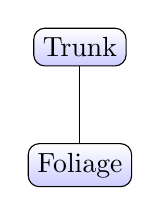
\begin{tikzpicture}[sibling distance=6em,
  every node/.style = {shape=rectangle, rounded corners,
    draw, align=center,
    top color=white, bottom color=blue!20}]]
  \node {Trunk}
    child { node {Foliage}};
\end{tikzpicture}
\\
Simply enough, we made trees that have different heights, and they are made in such a way that an iteration occurs over the creation where foliage gets added veritcally until we reach the desired height, so each cube of foliage is a child of the trunk.

TODO GLI ALTRI MODELLI!
%Descrivi gli altri modelli hierarchical: macchine, terreni, tronchi sul fiume, cespugli

%ogni personaggio, auto, tree, ambiente(River, Road) (ricorda che hai track --> tree/auto (sono figli del track))
\subsection{Lights and Shadows}
%parla della luce del sole (con i dettagli della luce scelta), la luce del lampione (con alternanza giorno notte)
%distinzione tra receive shadow and cast shadow e dove le hai attivate e dove no e perchè
Now we are going to talk about lights and shadows organization in the game and how they impact on the performance of it. In particular we will discuss what the user can see in the space and how the objects interact with them. 

First of all, in the game the user has the possibility to choose playing in night mode or day mode and, according to the choice made by the him, we find different sources of light:
\begin{itemize}
  \item Day, when we set the day mode the unique source light is the sun. Basically we use a SpotLight with with the following characteristics:
  \begin{lstlisting}
    spotLight = new THREE.SpotLight( 0xffffff, 1 );
    spotLight.penumbra = 0.05;
    spotLight.decay = 2;
    spotLight.distance = 500;
    spotLight.angle = Math.PI / 4;
  \end{lstlisting}
  We used this type of light because it's perfect to simulate a sunset, that is better to exploit the water's reflection properties due to the greater angle of the light;
  \item Night, in the night mode we have a street lamp in the starting point of the game. Also in this case we used a SpotLight object, but this time we decrease the angle of it (because of course a lamp can't have the same range of the sun) and we decrease the intensity of it:
  \begin{lstlisting}
    this.spotLight = new THREE.SpotLight( 0xffffff, 0.6 );
  \end{lstlisting}
  The initial idea was to add headlights to every car, but due to the very high number of cars in the game this would have brought to some performance slowdowns in some cases, so the discarded that idea. 
\end{itemize}
In addiction to the SpotLights we also added an ambient light in order to a better distribution of the light, specially in night mode:
\begin{lstlisting}
  ambientLight = new THREE.AmbientLight( 0xffffff, 0.6 );
\end{lstlisting}
the latter is the ambient light during the night. For the day we have the same object but with a greater intensity equal to $1.1$. Here we report an image of the street lamp in action generating also some shadow.

\begin{figure}[!h]
  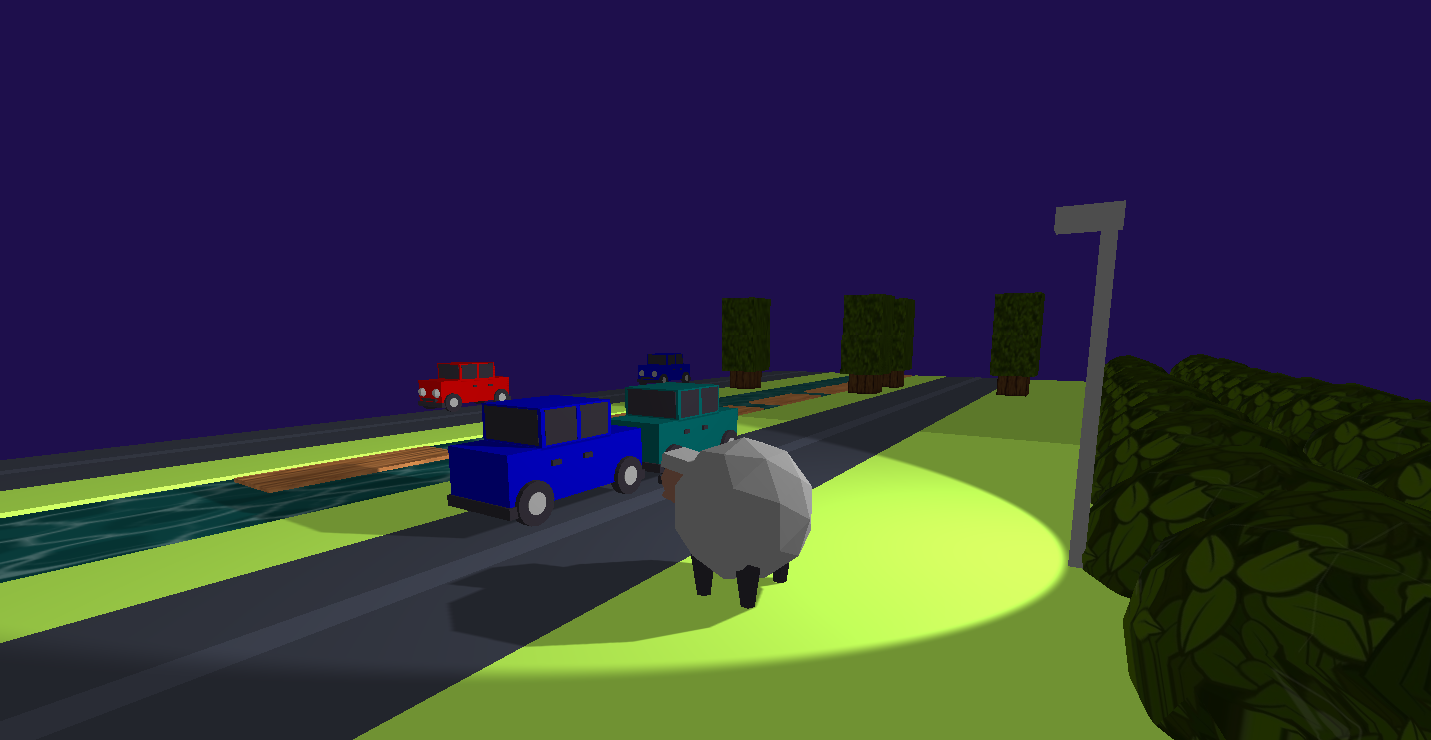
\includegraphics[scale=0.25]{lampShadow.png}\\
\end{figure}

About that, the second aspect of the project related to lights are shadows. These are very important in order to make more realistic the animation and the scene, but at the same time they are very heavy in terms of computational power, specially without a GPU. So it's very important to find a compromise in terms of shadows' definition and details and performance. 

There are two options that can be added to every object and both add a functionality related to the shadow:
\begin{itemize}
  \item Receive shadow, this option allows the objects to receive the black color of the shadow. This isn't too heavy so can be added without any big trouble. Indeed we added it to every object in the game, but at the same time it's fundamental in order to visualize the shadows;
  \item Cast shadow, this other option instead enable the generation of shadow, simply denoting to Three js if the object have to block the light or not. This operation is very heavy indeed also in the documentation of the library is recommended to use with parsimony. So we added this function only to the main parts of the objects. 
\end{itemize}
In particular here we analyze what casts a shadow in the game and why:
\begin{itemize}
  \item The animals cast mainly the body, head and arts' shadow when they have them, without casting the shadow of little details like eyes, that produce an insignificant variation to it;
  \item Cars, due to the high number of them, cast only the body and the windscreen that are the two main component of the object. The other are only little details;
  \item Woods, they don't cast shadow because simply there isn't a plan when we shuold see their shadow, because they are floor's element;
  \item Trees, every part of them cast a shadow because they are very simple;
  \item Tracks, as for the woods, they don't cast shadow for the same reason.
\end{itemize}

\subsection{Texture}
Textures are the basis of most computer graphic applications.\\
Before starting this section, we will see three kind of textures we have applied to the same object in our project: the logs floating the river.\\
\begin{figure}[!h]
\minipage{0.3\textwidth}
  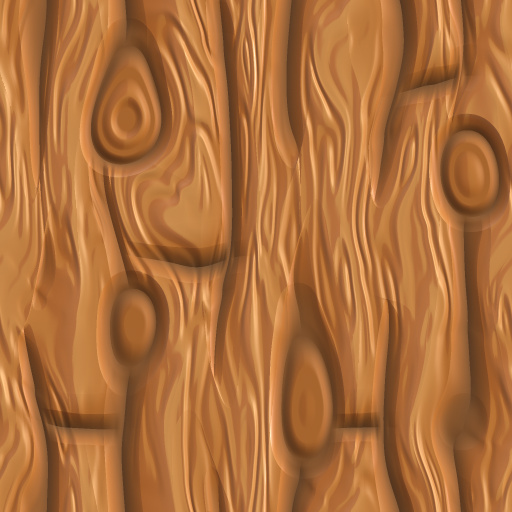
\includegraphics[width=\linewidth]{sidelog.jpg}
  \caption{Standard}\label{fig:tex_img}
\endminipage\hfill
\minipage{0.3\textwidth}
  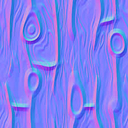
\includegraphics[width=\linewidth]{sidelognormal.jpg}
  \caption{Normal}\label{fig:n_img}
\endminipage\hfill
\minipage{0.3\textwidth}%
  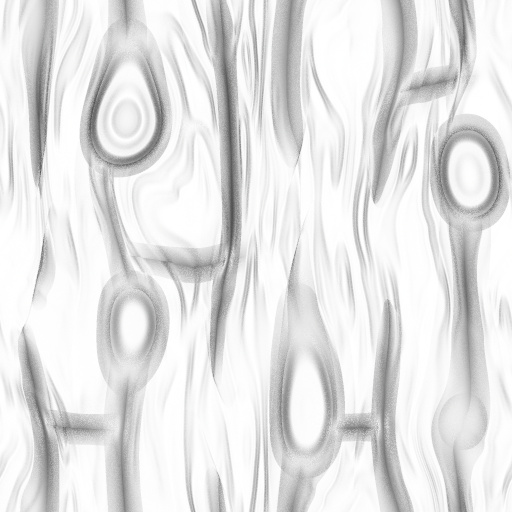
\includegraphics[width=\linewidth]{sidelogao.jpg}
  \caption{AO}\label{fig:ao_img}
\endminipage
\end{figure}
\\
In our game, we used the textures to give detail to our models, all images used are from free-of-use libraries and sites. Briefly, when using more than one texture on WebGL, they get composed(by multiplying the "n" textures) in WegGL's shaders.\\
A normal map texture is a texture which uses rgb values to signify the orientation of the surface normal by corresponding those values to the xyz of the surface normal at any given pixel. Basically it gives a lower-detailed model(e.g. a cube) finer details with respect to the interaction with the light. In our project we've decided to add them only to two objects:
\begin{itemize}
\item Logs : in order to make the logs more realistic(and as a collateral, more "dynamic") we've added to them a normal map. But since they are made of wood, they should not reflect much light and thus we made them a MeshPhongMaterial, which is a three js material which won't shine as much as the Lambert one. While we were not using the Phong material, it was reflecting an absurd amount of light with the normal mapping active and would've been an extremely realistic effect on most other materials.
\item Foliage and Bushes : in nature, most trees' crown and most king of bushes shine under the light, we applied a normal map to capture this shininess.
\end{itemize}
And ambient occlusion(AO) texture is used to add shadow details to the object it is applied to, pronuncing its effects and giving a better sense of depth.
The decision to not apply textures to all our object was agreed by all the members because after approaching the state that can be seen in the repo, all subsequent texture implementation were making the project look worse, less sharp and more messy than it needed to be. For this reasons we didn't put any texture on the animals or the ground.\\
Also in the case of the water, we tried different combinations of Texture/Normal Texture, but the final one without any normal mapping was way better looking than any other combination and since we already had normal textures in the project it didn't seem a good idea to make it worse purposely.\\
\subsection{Animals animations}
Each of our animations has been hand-made by us over the hierarchical models we've implemented and then animated.\\
Since they are all quite similar, we will analyze the most complex and articulate one : the Fox.\\
\begin{center}
	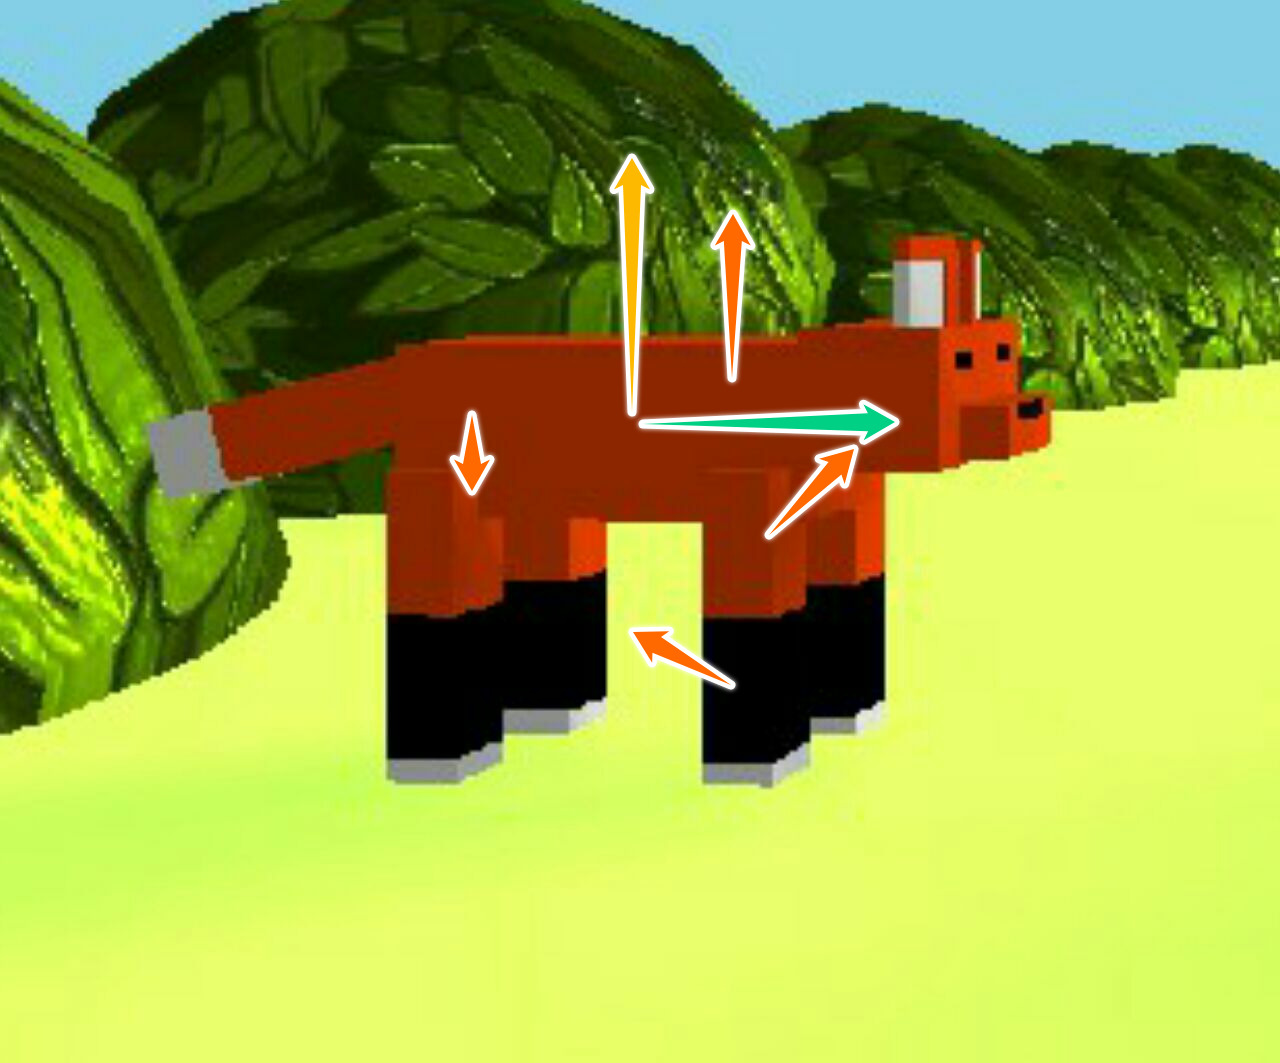
\includegraphics[scale=0.2]{FoxAnimation.jpeg}\\
\end{center}
In the previous figure, the orange arrows represent the rotations(with respect to the x axis going in the opposite direction from the viewer towards the fox) which will affect the animal, namely the torso rotation upward, the upper leg and lower leg rotating in opposite direction. Furthermore the animal will traslate toward the directions it is facing, Z positives in our image, and upward in the Y axis.\\ When the Fox reaches the peak of its jump, it will suffer rotations opposed to the one we've described, in order to reset for the next jump, since it is simply the inverse of these, an image was deemed unnecessary.\\
Before doing all of this, when recognizing an input from the user, we check what key he has pressed and based on that we rotate the animal to do the correct jump.\\
As we were discussing, the Fox has the most complex animations, since we wanted a feel of simpicity for the sheep, and the chicken has inherently a simple jump. Thus the latters have parametric jumps where, by the use of trigonometric functions we apply rotations back and forth.\\
The fox is based on a counter animation. After noticing how many renders/jump functions were needed by the animal to conclude the jump animation, we divided the functions and in the first half we do the animation described in photo, while in the second part we do the exact opposite rotations to get back in place.\\
To compensate this complexity difference, the Sheep has also flapping ears which move when jumping and the Chicken flaps its wings.\\
Apart from the jump animations, all animals have two other animations:
\begin{itemize}
\item SunkAnimation: which happens whenever an animal falls in to the river. This animation shows the animal sinking(dropping hastly along the y axis) and a splash effect starts, which prompts the creation of splash particles(squares of the same color of the river, for simplicity) that rise and fall from the point of sinking.
\item CrashAnimation: happens whenever a car and the animal comes in contact. We wanted to achieve a rather humurous effect, in fact the animal gets propelled toward the air way faster than it should be, while rotating along two different directions. The details of how the detection happens will be explained in the next section.
\end{itemize}
All animations were done by using the hierarchical model of the animals and then using three js's function:
\begin{itemize}
\item : object.rotation.axis : which sets/offsets the rotation of an object along one axis  by a certain angle in radiants.
\item: object.rotateOnAxis(new Axis), which is used to rotate correctly along the original axis when the animal is rotated(and thus has its relative axis moved).
\end{itemize}
%anche l'animazione dello splash, nella sezione successiva parliamo solo della detection
%animazione degli animali, animazione auto/trunk, animazione sunk, animazione crash
\subsection{Vehicles animation and object detection}
The other two classes of objects moving are the cars and the logs on the rivers.\\
Simply enough, both of these move along the x axis, either with it or in the opposite direction. Since we wanted a minimalistic approach and we have given to all the cars black tires, we noticed that making the tires rotate had no visible effect and was only stressing the  processing so we scrapped that animation.\\
%parla sia del crash con auto, splash del personaggio e detection dei trees/bush
\subsection{Optimizations}
%parla dell'uso dei Layers e delle animazioni che partono solo quando il personaggio si avvicina
%
%how much they increase the perfomance
%riporta la disposizione dei valori label dei livelli
In these section we are going to analyze the optimization techniques adopted in the project and how much they increase the perfomance of the game. \\

The first optimization was added using a layered organization of the random map. Indeed, at the beginning of the development we start spawning all the tracks (River or Road) in the init function and then rendering all of them (consequently also their children element) for every frame. Obviously, this may bring to some slowdowns, specially in computers without GPU. 

So, in order to resolve the issue, we simply render only the tracks that are close to the animal, in particular the tracks that are visible from the camera. 
This is done using Layer, an module provided by Three js, that allow us to label every element in the game with a value. The latter is used by the camera to know if it must render an object or not. Indeed, by default every object in the space (camera included) have value zero, as if it is a unique layer. 
Hence, in order to render a limited number of tracks $n$ in each frame, we need to assing the labels so that every track is visible for $n$ layer. The following is an example of $n=4$ that should clarify how to do it:
\begin{equation}
    \begin{array}{lllll}
	Track3: & 1 & 2 & 3 & 4\\
	Track2: & 0 & 1 & 2 & 3\\
	Track1: & 0 & 1 & 2\\
	Track0: & 0 & 1
    \end{array}
\end{equation}
if the camera is set to layer $2$ we will see tracks number $1,2,3$.
Of course in the code we find a parametric code that assign the label correctly, using the variable called $numOfLevelVisible$.
Then of course the camera need to increase its value every time the animal come near a new layer as we can see in the render function:
\begin{lstlisting}
	if(referencePositionAnimal.z > limitMax){
		actualLevelCamera++;
      	camera.layers.set(actualLevelCamera);
	}
\end{lstlisting}
here the label of the camera is increased every time the animal reach a new layer. 

The same idea is used also for cars and trunks' animations. Indeed, their movements starts only when the player is close to the track (in particular it starts only for the current, next and previous track). In order to do that we use the previous check to know if we need to update the data structure that contains all the active tracks in the game, called $actualListTracks$. Then it will used by the fuctions that animate them, scanning a fewer number of tracks. Also this optimization is adopted by the trees detection because they are child of the tracks, so they are affected by the activation of only a part of them. 
Of course if the animal try to go back there is a piece of code that decrease the camera's label and load the old tracks previously cross. \\

The final result is a more fluid game, in our tests we passed from 20 fps to 50 fps in similar map situations. 


\section{User-game interactions}
We will explain how the interactions are implemented. UI elements are skipped since they are simple html/js functions setting up flags and activating part of main code.
\subsection{Movement}
We use a javascript function(visible in crossyRoads.js) onKeyDown to check if any between A,S,W and D has been pressed. Then each animal has an actionOnPressKey which responds differently based on the key pressed. We will present the code for the press of W for the Sheep, some of the more wordy parts have been replaced by pseudocode, the full js code can be seen in the repository.
Start jumping:\\
\begin{lstlisting}
  actionOnPressKey(referencePositionAnimal) {
    if(inMotion){
      //continue the jump until its end
      this.jump(<params previously saved>);
    }
    else{
      if (keyWDown){
        checkTrees();
        //check if any tree is obstructing the jump, if true, don't move
         currentScore++;
        //Resetting parameters and preparing for inMotion
        inMotion = true
        this.jump(speedSheepUp, dist, 0, 'z');
        }
      }
     //other keys
\end{lstlisting}
Jump function:
\begin{lstlisting}
  jump(speed, dist, gradi, ax) {
    this.group.rotation.y = rad(gradi);
    this.vAngle += speed*goingFastSheep;
    //check if jumping up or down, keep moving or switch it if
    //jump peak reached
    checkJump();
	
    //rotations were done with trigonometry and arbitrary parameters.
    const legRotation = Math.sin(this.vAngle) * Math.PI / 6 + 0.4;
    applyRotation(legs);
    //check the direction and slightly move the animal accordingly
    moveForward(ax);
    const earRotation = Math.sin(this.vAngle) * Math.PI / 3 + 1.5;
    applyRotation(Ears);
    //check if the jump has to end
    if(this.group.position.y <= 0.4){
	  resetFlagsAndHeight();//inMotion = false is the most important
	  //update the score which is seen in the higher part of 
	  //the screen only if we are moving toward the goal
      if(ax=='z') {
        if(sign == 1){
          document.getElementById("cScore").innerHTML = currentScore;
          if(currentScore > highestScore){
            highestScore = currentScore;
            document.getElementById("hScore").innerHTML = highestScore;
          }
        }
  }
\end{lstlisting}
\subsection{Camera}
As it can be seen in game, the camera starts going forward as soon as the user make a jump forward. And it keeps on going forward until either a game over or a win occurs also due to the user being able to outrun a lot the camera in the easier difficulties, the movement is parametric to the distance between the camera and the animal positions.
\begin{lstlisting}
  if(highestScore == numberOfJumpsToDo){
    //reached the goal, stop the game and output victory screen
    flag = false
    eventMsg("You Win!");}
  if(!flag){
    if ((tot > referencePositionAnimal.z + 1.5 ) ||
      (referencePositionAnimal.x.isOutOfBounds){
      //Animal got out of the viewable area, game over
      stopGame();
      eventMsg("Outrunned!");
    }
    //move only if user jumped at least once forward
    else if(highestScore != 0){
      if(referencePositionAnimal.z - tot >= 0){
        //setUp the camera based on the distance with the animal
        tot+=diffModifier*(1+ (referencePositionAnimal.z - tot)/4);}
    }
    camera.position.set(0, 15, tot); 
\end{lstlisting}
This is done in the render position, meaning that at each frame rendering, the camera gets pushed forward and the conditions regarding win or lose status gets updated and checked.
\subsection{difficulty}
The following table describes all values that get modified when changing difficulty. The relative code can be seen in crossyRoad.js in the 	setDifficulty(difficulty) function.
\begin{table}[h]
\begin{tabular}{c|c|c|c|}
\cline{2-4}
\multicolumn{1}{l|}{}                                  & \textbf{Easy}             & \textbf{Medium}      & \textbf{Hard}        \\ \hline
\multicolumn{1}{|c|}{\textbf{Number Of Levels}}        & 6                         & 10                   & 16                   \\ \hline
\multicolumn{1}{|c|}{\textbf{Number of Cars}}          & {[}0,2,3{]}               & {[}1,2,3{]}          & {[}2,3,4{]}          \\ \hline
\multicolumn{1}{|c|}{\textbf{Speeds of Cars}}          & {[}0.04,0.05,0.05,0.12{]} & {[}0.06,0.08,0.15{]} & {[}0.15,0.18,0.25{]} \\ \hline
\multicolumn{1}{|c|}{\textbf{Speeds of Logs}}          & {[}0.01,0.02,0.05{]}      & {[}0.03,0.04,0.1{]}  & {[}0.05,0.06,0.13{]} \\ \hline
\multicolumn{1}{|c|}{\textbf{Camera's speed modifier}} & 0.035                     & 0.04                 & 0.05                 \\ \hline
\end{tabular}
\end{table}
Number of levels changes the number of terrain alternation that gets generated between start and goal.\\
Speed of cars and logs are two lists used when creating such vehicles. A random function is applied and each line of vehicles has then a different speed.\\
Camera's speed modifier can be seen in the last part of the previous code defining the base speed of the camera moving forward.

\end{document}
